%\documentclass[letterpaper, 10 pt, conference]{ieeeconf}  % Comment this line out
                                                          % if you need a4paper
\documentclass[a4paper, 10pt, conference]{ieeeconf}      % Use this line for a4
                                                          % paper

\IEEEoverridecommandlockouts                              % This command is only
                                                          % needed if you want to
                                                          % use the \thanks command
\overrideIEEEmargins
% See the \addtolength command later in the file to balance the column lengths
% on the last page of the document
\providecommand{\tabularnewline}{\\}
%% Because html converters don't know tabularnewline

% The following packages can be found on http:\\www.ctan.org
%\usepackage{graphics} % for pdf, bitmapped graphics files
%\usepackage{epsfig} % for postscript graphics files
%\usepackage{mathptmx} % assumes new font selection scheme installed
%\usepackage{times} % assumes new font selection scheme installed
%\usepackage{amsmath} % assumes amsmath package installed
%\usepackage{amssymb}  % assumes amsmath package installed
\usepackage[utf8]{inputenc}
\usepackage[T1]{fontenc}
\usepackage{graphicx}
\usepackage{textcomp}
\graphicspath{ {images/} }


\title{\LARGE \bf The correlation between Smart-cities and gentrification }

\author{Jérémy Scheurer, Philipp Miotti and Rob Spaargaren}

\begin{document}

\maketitle
\thispagestyle{empty}
\pagestyle{empty}


%%%%%%%%%%%%%%%%%%%%%%%%%%%%%%%%%%%%%%%%%%%%%%%%%%%%%%%%%%%%%%%%%%%%%%%%%%%%%%%%
\begin{abstract}
%Note in the whole text we will write Smart with a capital S. Because we want to make clear that we are not talking about the adjective smart but aobut a term that has been coined with defining the technologica progress of a city. 

%Maybe mention that our contribution is also a novel dataset with distances and household incomes for international cities. 

Quick summary of goal and results. 

\end{abstract}


%%%%%%%%%%%%%%%%%%%%%%%%%%%%%%%%%%%%%%%%%%%%%%%%%%%%%%%%%%%%%%%%%%%%%%%%%%%%%%%%
\section{INTRODUCTION}
\label{sec:Introduction}
The technological progress of our society shapes our daily life in an unprecedented
way and faster than ever before. Since the introduction of the internet, our world 
has become progressively more connected and new ways of collecting data are introduced
continuously. This data is used to implement new systems to improve the quality of life.
Following this trend, modern sensors are deployed in cities to communicate with systems
(e.g.\ public transport or parking sensors) to improve the functioning of these systems 
and offer high quality services to the citizens. A city that deploys many of these systems
to improve the general quality of life of its citizens is called a Smart city.

A city which develops itself to a Smart city greatly increases the living standard
for its citizens, making it more attractive for people to move there. This spurs an 
influx of wealthy inhabitants, who also move into the poorer districts of the city,
since these districts also experience a great increase in quality of living. These new,
wealthy inhabitants invest money to increase the quality of their neighbourhood even further,
leading to increasing living costs, driving out the poorer former residents. This 
process of wealthy inhabitants moving in a neighbourhood, investing money to renovate
the neighbourhood, increasing the living quality and living costs and
driving out the poorer former residents, is called gentrification. Therefore, 
there might be a link between gentrification and the development of cities to become Smart.
The importance of investigating this link lies in the possibility for cities to pre-emptively
change their policies to protect the poorer residents and prevent the neighbourhoods these
citizens move into from deteriorating.

To investigate whether this link exists, a quantity indicating the Smartness
of a city should be compared to a quantity characterizing the degree of gentrification
of the city. To give an indication of the smartness of a city, we will use two publicly
available rankings of cities across the globe. The ranking of a city across both lists
is used as an indicator of the Smartness of the city. The list we have used are published
by the IESE Business School of the Universtiy of Navarra \cite{c1}, and by the Easypark group \cite{c2},
an international group specialising in implementation of smart parking in cities.

Initially, gentrification was defined by Ruth Glass in 1964 as the displacement of lower-class
working residents in urban neighbourhoods by middle-class citizens \cite{gentr_def}. This definition
is not useful to quantitatively measure gentrification, so the wide effects of gentrification on a neighbourhood should be utilized.
There is a wide variety of effects of gentrification on the neighbourhood, which could be used
to quantify it. The nature of the neighbourhood changes, affecting not only housing prices and
living costs, but also the look of the neighbourhood, by increasing the amount of public green
and parks, and the number of schools. Gentrification also induces a shift in demographics, in
culture, educational level and household income. These effects have been used in both qualitative
and quantitative research (see Barton, 2016, for an overview \cite{Barton}). However, the changes
in neighbourhood characteristics could be due to a number of other factors like a change of policy
by the city government rather than gentrification, and can be subjective of nature. Of the effects
on characteristics of the population, an increase of income is the most indicative and least 
subjective sign of the transition to a higher social class. Using a quantity based on household
income to measure gentrification has also been used in other quantitative studies \cite{gentr_research}.
We present a metric based on the Gross Disposable Household Income (GDHI) that quantifies gentrification
in this paper.

%Add another paragraph! Describe data collection and why we used a data science approach.
%Mention database on gitlab and additional importance of presenting the dataset.
%Maybe mention the paper of the stanford guys...and the paper which looked at gentrification in 7-8 american cities. 

\section{Gentrification Index as a metric}
\label{sec:Gentrification}
% Should be best done by philipp 

% First describe our procedure 1. we want to make difference between smart and non smart-cities
% 2. We need to calculate a gentrification index. for that we need distances and income

%TDescribe our novel approach on how we came up with our gentrification measurment. 
%Much of it can be taken from the mini paper of Philipp. Note philipp that you should probably recalculate your stuff
%you did wiht different years. In your mini paper you compared 2016 to 2007...but in our database we are using 2016-2008...
%just for the sake of completion. If you have no time never mind. 

% This section should be the heart of our paper!!! it has to argue convincingly why this metric which uses districts of a city
%shows the gentrification of a city. You can stay general. I will gon itno the details about how we defined these districts etc. in the next section.

To quantify gentrification, we have developed a metric based on the GDHI of different districts of a city, which meets certain requirements.
Firstly, we require our metric to be independent of the initial state of a city (temporal independence),  i.e., to capture merely the
gentrification in a certain timespan irrespective of the mutual differences between city parts at an initial time from which the analysis
has started. Moreover, it should be possible to compare the extent of gentrification for various cities from all over the world (spatial independence).
Thus, we have to make it independent of the local currency and of the overall wealth of a city. In addition, a weighting shall be applied to the
neighbourhoods based on their distance. Differences between adjacent and close neighbourhoods will be weighted more heavily than differences between
those that are far apart, as the notion of gentrification tries to capture local distinctions. Lastly, we require it to be a 
non-negative, strictly increasing, and intensive quantity. The last properties imply that the index is zero, if all districts have the same GDHI, 
and it increases, if the income gap also increases. Intensiveness of our metric means that the it does not scale with the size of the city or with
the number of districts.

We propose the change of the GDHI with respect to time as our central quantity to derive our metric. The change of GDHI is compared between the different
districts of a city, where the division of a city into districts is  by virtue of administrative division units ADU. To study the temportal change of GDHI
between different districts across the same timespan, to avoid noise induced by different conditions prevalent to different times, we compared the data of
each district in the timespan 2008-2016. How the units for a particular city were actually chosen is described in section \ref{section:Data}.
To assure temporal independence, we calculate the increase of the GDHI in each ADU $x_{i}=x(District = District i)$ relative to the increase of the GDHI 
averaged over the whole city, $\tilde{x}$. More precisely, 

\begin{equation}
\begin{split}
x_{i}=\frac{\mathrm{GDHI}(i,2016)-\mathrm{GDHI}(i,2008)}{\mathrm{GDHI}(i,2016)}, \\
\quad\tilde{x}=\frac{\widehat{\mathrm{GDHI}}(2016)-\widehat{\mathrm{GDHI}}(2008)}{\widehat{\mathrm{GDHI}}(2016)},
\end{split}
\label{eq:gdhi}
\end{equation}

where $\ \widehat{}\ $ denotes the average of GDHI in a particular year over all districts $i$. To normalize this increase of income
in district $i$ with respect to the increase of income of the rest of the city, and to make it independent of valuta and other city-specific
factors, we will use $r_{i}=\left(x_{i}-\tilde{x}\right)/\tilde{x}$ in our metric. Tab.$\,$\ref{tab:Median-household-income} shows this relative
increase of the GDHI in case of Berlin, which suits as an example to demonstrate our metric. Two normalizations were used in the above definitions: 
one in $x_{i}$ or rather $\tilde{x}$, and the other in $r_{i}$.
Because an absolute gentrification is not sensible, we have to choose relative variables for our gentrification measure. 
The contribution of the first is twofold; we normalize the GDHI to a specific arbitrary year. This corresponds to a temporal 
normalization. Without the second ''spatial'' normalization, we would not be able to compare the cities with each other. 

\begin{table}[h]
	\begin{centering}
		\begin{tabular}{|c|c|c|c|}
			\hline 
			District & $\mathrm{GDHI}(i,2008)$ & $\mathrm{GDHI}(i,2016)$ & $r_{i}$ \tabularnewline
			\hline 
			\hline 
			$1$ & $22000$ & $27900$ & $-0.14$\tabularnewline
			\hline 
			$2$ & $18000$ & $21300$ & $-0.37$\tabularnewline
			\hline 
			$3$ & $17700$ & $25500$ & $+0.25$\tabularnewline
			\hline 
			$4$ & $19600$ & $24300$ & $-0.21$\tabularnewline
			\hline  
			$5$ & $16200$ & $21900$ & $+0.05$\tabularnewline
			\hline 
			$6$ & $18800$ & $23700$ & $-0.16$\tabularnewline
			\hline 
			$7$ & $14800$ & $21600$ & $+0.27$\tabularnewline
			\hline 
			$8$ & $17400$ & $25800$ & $+0.32$\tabularnewline
			\hline 
			$9$ & $15500$ & $20400$ & $-0.02$\tabularnewline
			\hline 
			$10$ & $17400$ & $21900$ & $-0.17$\tabularnewline
			\hline 
			$11$ & $17700$ & $23400$ & $-0.01$\tabularnewline
			\hline 
			$12$ & $17800$ & $24600$ & $+0.13$\tabularnewline
			\hline 
		\end{tabular}
		\par\end{centering}
	
	\caption{Median household income per month in EUR in Berlin (city divided into
		districts according to Figure \ref{fig:map_berlin}) in years
		2008 \& 2016, along with normalized increase of income $r_i$.}
		\label{tab:Median-household-income}
\end{table}


\begin{figure}
	\centering{}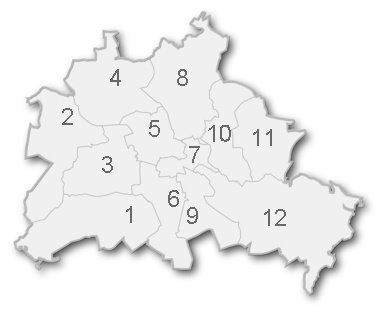
\includegraphics[scale=0.6]{stadtplan-berlin}
	\caption{Map of Berlin's districts with random numbering. Image: © Increa}
	\label{fig:map_berlin}
\end{figure}

The next step consists of defining a measure for the distance of a district with respect to each other. 
A generic solution is to use the ADU structure of an city, the districts themselves as distance units. 
Therefore, we introduce the number of minimal district-border-crossings, which are necessary to get from 
district $i$ to district $j$, as our distant measure. For example, the distance, denoted as $\left\langle \cdot,\cdot\right\rangle $,
of district 1 to district 8 in Fig.$\,$\ref{fig:map_berlin} is equal to 3, i.e. $\left\langle 1,8\right\rangle =3$.
Hence, differences in the values $r_{i}$ of district further apart contribute less to the gentrification index $g_{i}$
of an particular district $i$. For the sake of intensiveness we have to normalize this distance by the total number of 
districts in a city. How the distances are calculated exactly is explained in section \ref{section:Data}.

The final step consists of putting the quantities $\left\langle \cdot,\cdot\right\rangle $ and $r_{i}$ together 
in a way which results in a meaningful formula for gentrification satisfying our requirements, 

\begin{equation}
G=\sum_{i=1}^{N}G_{i},\quad G_{i}=\frac1{N}\sum_{j=1,\,j\neq i}^{N}\frac{\left|r_{i}-r_{j}\right|^{2}}{\left\langle i,j\right\rangle },
\label{eq:gindex}
\end{equation}
We call $G$ and $G_{i}$ the gentrification index of a city and the gentrification index of the city district $i$ respectively. Due to the fact that gentrification is a rather subjective notion, and the fact that in the perspective of citizens it manifests itself the most when adjacent neighborhoods are compared, we divide by our distance measure $\left\langle \cdot,\cdot\right\rangle $. This has the effect to soften the differences between two districts when they are far apart. The meaning of the numerator in Eq.$\,$(\ref{eq:gindex}) is clear when we write out the squares, $\left(x_{i}^{2}-x_{j}^{2}\right)/\tilde{x}^{2}.$ The numerator is smaller, if the mean GDHI of the city $\tilde{x}$ is high. Then, two district with a big difference in the GDHI $x_{i}-x_{j}$ are going to make $G_{i}$ small, whereas on those where the difference is small $\tilde{x}$ has no effect at all. With this feature we can take into account the overall increase of the GDHI in a city. The gentrification index of an city with a low $\tilde{x}$ but a distinctive shift of citizens of different working-classes shall be especially big, as we can then assume that wealthier people haven't moved in from beyond the city at an above average rate.

Where $N$ is the number of districts in the city.
We call $G$ and $G_{i}$ the gentrification index of a city and the gentrification index of district $i$ respectively.
Due to the fact that gentrification is a rather subjective notion, and the fact that in the perspective of citizens it manifests 
itself the most when adjacent neighborhoods are compared, we take the square of our distance measure $\left\langle \cdot,\cdot\right\rangle $.
This has the effect to soften the differences between two districts when they are far apart. The meaning of the numerator in Eq.$\,$(\ref{eq:gindex})
is clear when we write out the squares, $\left(x_{i}^{2}-x_{j}^{2}\right)/\tilde{x}^{2}.$ The numerator is smaller, 
if the mean GDHI of the city $\tilde{x}$ is high. Then, two district with a big difference in the GDHI $x_{i}-x_{j}$ are going 
to make $G_{i}$ small, whereas on those where the difference is small $\tilde{x}$ has no effect at all. With this feature we can 
take into account the overall increase of the GDHI in a city. The gentrification index of an city with a low $\tilde{x}$ but a distinctive 
shift of citizens of different working-classes shall be especially big, as we can then assume that wealthier people haven't moved in from 
beyond the city at an above average rate.

Although, the above argumentation is sensible, we can't be sure if Eq.\ \ref{eq:gindex} is the best formula for the index. Thus, we also present
some alternatives to $G_{i}$, and compare these to the equation. Namely, 

\begin{equation}
\begin{array}{cc}
G_{i}^{\prime}= & \sum_{j=1,\,j\neq i}^{N}\frac{\left|r_{i}-r_{j}\right|^{2}}{\left\langle i,j\right\rangle ^{2}}\\
G_{i}^{\prime\prime}= & \sum_{j=1,\,j\neq i}^{N}\frac{\left|r_{i}-r_{j}\right|}{\left\langle i,j\right\rangle ^{2}}\\
G_{i}^{\prime\prime\prime}= & \sum_{j=1,\,j\neq i}^{N}\frac{\left|r_{i}-r_{j}\right|}{\left\langle i,j\right\rangle }
\end{array}.
\label{eq:gindex_alt}
\end{equation}
Tab.$\,$\ref{tab:Correlation} shows the correlation between the gentrification indexes in each district and the quantities $r_{i}$ for the various types of $G_{i}$, and the gentrification index $G$ as well. Based on this results we propose the formula in Eq.$\,$(\ref{eq:gindex}) as our best measure for the gentrification of a city.

\begin{table}[h]
	\begin{centering}
		\begin{tabular}{|c|c|c|c|c|}
			\hline 
			$G$ & $0.66$ & $0.51$ & $1.42$ & $1.82$\tabularnewline
			\hline 
			\hline 
			$\mathrm{corr}\left(\cdot,\cdot\right)$ & $G_{i}$ & $G_{i}^{\prime}$ & $G_{i}^{\prime\prime}$ & $G_{i}^{\prime\prime\prime}$\tabularnewline
			\hline 
			$\left|r_{i}\right|$ & $0.98$ & $0.96$ & $0.93$ & $0.94$\tabularnewline
			\hline 
		\end{tabular}
		\par\end{centering}
\caption{Correlation between the different gentrification indices of Equation \ref{ew:gindex_alt}.}
\label{tab:Correlation}
\end{table}



\section{Data}
\label{section:Data}
%Done by Jeremy but please review and change afterwards...its not perfect
%1. Describe what database we use and why 
%2. Describe how you gathered data 
%3. Describe how you filled up empty spots
%4. Describe how you regressed data 
%5. A plot which shows what years we actually had data on and what years were regressed
%6. Argue why taking cities which were not on the list is ok
As described before, our goal consists of comparing a gentrification-index of Smart-cities and Non-Smart-cities. 
Our first challenge lies in defining which properties make a city Smart or Non-Smart. Secondly we need to calculate
the gentrification index which requires the following: 

\begin{enumerate}
	\item  Data on the average houshold income per district of a city
	\item Data on the distances between districts of a city 
\end{enumerate}

In this section we will proceed by explaining our data gathering process for both challenges. 


\subsection{Smartness of a city}
We explained in our introduction how the term smart city is defined. Also intuitively it is easy to imagine the properties
that a smart city can have. Things like a car sharing servics, universal wifi access, a digitalized government, efficient public transport,
clean energy generation and much more come to our minds. But to quantitatively asses if a city is smart or not, which means to look at 
all properties, weigh them accordingly and combine them into a single index, is a very non-trivial task. It would have been out of the 
scope of our work to attempt to figure out some way of quantizing the Smartness of a city, colllect enough data and create a ranking.
We are thus using the smart city rankings of [1] and [2] which use the following criteria to create their rankings:\newline

\begin{itemize}
\item [1] is based on 66 different indicators, subdivided in 10 dimensions:
Human capital, social cohesion, economy, public management, governance, mobility and transportation, environment, urban planning, international outreach and techonology.
\item [2], an international group specialising in implementation of smart parking in cities, have created a ranking based on transport and mobility, sustainability, governance, innovation economy, digitalisation, living standards and expert perception.
\end{itemize}
% Here is a mistake...how can i make the [] visible after the itemize

The remaining question is how to combine these two rankings when trying to decide between Smart-cities and Non-Smart-cities. 
When looking at both raknings we can make out, that cities which are ranked in the top Smart cities of one ranking,
oftentimes are also ranked as top Smart cities in the other ranking (see table x). Because we lack a ground-truth with 
which we could compare both rankings, it is very difficult to reason about the differences and about how they come about. 
Thus we are left only with our intution on which ranking we could trust more. Obviously [1] has several years of experience in 
producing his "Cities in Motion Index", he also goes into much depth about what properties are relevant for the ranking and why.
Finally the university produces an extensive, yearly report about the current rankings. In comparison [2], as a smart parking company, 
has also much experience in the field and lists all its factors that weigh into the ranking. But on the other hand they go much less
into the details of how and why they chose these properties. To sum up, [1] makes definitely a more thorough impression than [2]. 
But nevertheless [2] is rigorous enough in its analysis, that we decided to keep it aswell as a reference for the Smart-city ranking.
Thus for this study we defined a smart city the following way: \newline
\textit{A Smart-city, is a city which is ranked in the Top-20 of the Smart-city rankings of [1] and [2].}

\includegraphics[scale=0.5]{"images/rankings"}

For the sake of this paper, we wanted to make the difference between the Smart-cities and the Non-Smart-cities as large as possible.
Thus we wanted to define the Non-Smart cities as those which are ranked in the last 20 cities of the rankings of [1] and [2]. 
Unfortunately we did not find any data on the average houshold income per district of cities like Karachi(Pakistan), Lagos(Nigeria)
and others which were at the bottom of the rankings. Because we did find detailed datasets with very high granularity and coverage
for countries like the USA and Australia, we choose our Non-Smart cities from these countries. Specifically, we chose cities from
these countries which were not listed on the ranking of either [1] or [2] (there were unfortunately no US or Australian cities which
were ranked much lower than the Top-20 in either ranking). We argue that this is a reasonable choice for the following reasons. The
cities we chose belonged to the largest ones in their corresponding countries, thus one cannot argue that they were purely excluded
from the rankings because they were too small and thus not significant. Naturally one could argue that the only reason they did not
include these cities is because they did not find any data on them. One could even go further and propose that one of these cities, 
which we define as Non-Smart, could be in the Top-20 of on e of the the Smart cities rankings. To such an argument we would reason, 
that by creating such a ranking depending on different properties of cities, by researching what influences the "Smartness" of a city
and doing this for several years(this is at least the case for [1]), one could be considered as an expert in the field. And as expert 
in a field, one could have a good intuition on which city could possibly be a Top Smart-city and which not. Thus it is very unlikely 
that any of these cities, which are not on the ranking, actually would be a Top-20 city. Because if they were, [1] and [2] would most 
likely have included them in the ranking. (NOTE I AM INCLUDING THIS WARNING ON PURPOSE IN THE TEXT...THE FOLLOWING ARGUMENT CAN ONLY
STAY IN HERE IF OUR RESULTS ACTUALLY SHOW A STRONG DIFFERENCE IN GENTRIFICATION BETWEEN SMART AND NON SMART CITIES). Lastly our results 
show a strong difference of the gentrification index of Smart-cities and Non-Smart-cities. This makes the case that the cities not 
ontained in the ranking, actually are Non-Smart Cities even more likely. 

\subsection{Household income and district distance}
For our analysis we need the average household income of a specific district in a city. For some cities the districts are exactly
defined by the database(this is mostly the case for European cities) and for other cities we looked at a concise area surrounding 
its center and defined that as the city(this was mostly the case for US and Australian cities).$^{1}$ It is worth mentioning that 
for all US and Australian cities we used postal codes as "districts" of a city, because they gave us the required granularity that
we needed(census tracts were too granular and county subdivisions not granular enough). For European cities(which are usually smaller)
having more granular districts was a common trait, thus we just took the districts as defined by the database. 

Obviously our household income data comes form very different sources. All of them are official publications form the corresponding 
cities or countries. Because of the diverse nature of this data, different methods might have been used to estimate the houshold income
for a specific district in a city. The data came also in different representations(mean and median), over different time periods(weekly
income, monthly income, and yearly income) and for different amount of years( see an overview in Table X). We do realize that we do need
to take these statistics with a grain of salt, as they are only estimates. Nevertheless they are the only available data to do any research
on. To get the average houshold income into a unified database we did the following preprocessing: 

\begin{enumerate}
\item If, for a district in a city, we did not have houshold income data for at least half of the years that data was provided, we removed this district from the database altogether. 
\item If, for a district in a city, we did not ahve houshold income data for some years(but (1.) did not apply), we manually completed the database in the following way: 
	\begin{enumerate}
	\item If we did have data for a previous and a later year, we took the average of the closest previous and closest later year and set the missing year to that. 
	\item If we did have data for a previous year but not for a later year, we set the missing year to the value of the closest previous year. 
	\item if we did have data for a later year but not for a previous year, we se the missing year to the value of the closest later year. 
	\end{enumerate}
\item Lastly extended our dataset to the years of 2008-2016. We need this timeframe to be able to asses the correlation of the Smartness of a city and its gentrification over a longer timeframe, as gentrification is an effect which can only be measured over a longer timeframe. To extend our available data to the mentioned timeframe we fitted a linear polynomial of degree 1 to our data with certain given years. We then just looked at the linear line through our data and calculated its value at certain timestamps we did not currently have data on(see more in Table xx)
\end{enumerate}

As mentioned before, our distance measure for districts is just the shortest path of a certain district to another through other 
districts. We calculated this manually for all districts in all cities and appended this to our database.$^{2}$

\thanks{$^{1}$ The actual area considered to be in a city can looked up on our gitlab(HERE WEBSITE?)}
\thanks{$^{2}$ Again the district maps we defined our distances from can be looked up on our gitlab.}
\newpage
\includegraphics[scale=0.6]{"images/data_overview"}




\section{Results}
\label{sec:Results}
%Show our results and interpret them. Is it what we wexpected 
% apply t-test or whatever statistical thingy


\section{CONCLUSIONS}
\label{sec:conclusion}
%ARe we happy with what we found out? What was the tricky part about this data...what could have gone differently. Quick summary of what we did 

\section{Further Work}
%If we had enough time what else could we have done? 
%In our case data was a limiting factor...we could have done better by having more international data, 
% more data from cities that were actually on the list as non-smart cities and more smart cities data. 
For a further improvement of the gentrification index we suggest to incorporate the change of the number of households in each district, and divide the gentrification of that particular district with this change. This also influences gentrification. If, for instance, rental fees increase but the number of household decrease in a certain area, then we can assume that several cheaper households were displaced by a few expensive ones. 


Bla

\addtolength{\textheight}{-12cm}   % This command serves to balance the column lengths
                                  % on the last page of the document manually. It shortens
                                  % the textheight of the last page by a suitable amount.
                                  % This command does not take effect until the next page
                                  % so it should come on the page before the last. Make
                                  % sure that you do not shorten the textheight too much.

%%%%%%%%%%%%%%%%%%%%%%%%%%%%%%%%%%%%%%%%%%%%%%%%%%%%%%%%%%%%%%%%%%%%%%%%%%%%%%%%



%%%%%%%%%%%%%%%%%%%%%%%%%%%%%%%%%%%%%%%%%%%%%%%%%%%%%%%%%%%%%%%%%%%%%%%%%%%%%%%%



%%%%%%%%%%%%%%%%%%%%%%%%%%%%%%%%%%%%%%%%%%%%%%%%%%%%%%%%%%%%%%%%%%%%%%%%%%%%%%%%


\begin{thebibliography}{99}

\bibitem{c1} Berrone, P., Ricart., J.E.\ (2017). \emph{IESE Cities in Motion Index}. Retrieved from IESE website: \url{http://www.iese.edu/research/pdfs/ST-0396-E.pdf}
\bibitem{c2} Easypark group 2017 Smart Cities Index (n.d.). Retrieved from \url{https://easyparkgroup.com/smart-cities-index/}
\bibitem{gentr_def} Ruth Glass (1964). London: aspects of change. London: MacGibbon \& Kee.
\bibitem{Barton} Barton, M.\ (2016). An exploration of the importance of the strategy used to identify gentrification, Urban Studies, Vol.\ 53, Issue 1, pp.\ 92-111.
\bibitem{gentr_research} Ding, L., Hwang, J., Divringi, E.\ (2016). \emph{Gentrification and residential mobility in Philadelphia}. Regional Science and Urban Economics, 61, \emph{38-51}.
%\bibitem{gentr_causes} Steve Holland, Gentrification: Causes and Consequences, Journal of Lutheran Ethics, Vol. 16, Issue 1, Jan 2016

\end{thebibliography}

\end{document}
